\documentclass[12pt]{article}
\usepackage[a4paper,margin=2.2cm]{geometry}
\usepackage{amsmath,amssymb,amsthm,mathtools}
\usepackage{hyperref}
\usepackage{cleveref}

\usepackage{fontspec}
\usepackage{xeCJK}

\usepackage{fontspec}
\usepackage{xeCJK}
\setCJKmainfont{Noto Serif CJK SC}

\usepackage{tikz}
\usetikzlibrary{calc}

\title{Householder Reflection}
\date{}
\begin{document}
\maketitle


\begin{flushleft}
    1: 反射不是投影
    向量 v : \\
    \begin{align}
        v  \in  \mathbb{R}^{m}
    \end{align}
    它决定了一个超平面 :\\
    \begin{align}
        v^{\perp} = {x \in \mathbb{R}^{m} : v^{T}x = 0 }
    \end{align}
    选定 v 是 "法向量" 所有与 v 成垂直关系的向量 x 的集($x \in \mathbb{R}^{m}$) 成为超平面 \\
    对于任意 x :\\
    \begin{align}
        x \in \mathbb{R}^{m}
    \end{align}
    将它分解为: \\
    \begin{align}
        x  = x_{\perp} + x_{\parallel}
    \end{align} \\
    其中: \\
    \begin{align}
        x_{\parallel} = proj_{v}(x)                                      \\
        = \frac{\vec{v}\vec{x}}{||\vec{v}||} \frac{\vec{v}}{||\vec{v}||} \\
        = \frac{\vec{v}\vec{x}}{||\vec{v}||^{2}} \vec{v}                 \\
        = \frac{v^{T}x}{v^{T}v} v                                        \\
        = \frac{vv^{T}}{v^{T}v} x                                        \\
    \end{align}
    而: \\
    \begin{align}
        x_{\perp} = x  - x_{\parallel} (x_{\perp} \in v^{\perp})
    \end{align}

    这里我们要关注一些细节: \\
    \begin{align}
        x_{\parallel} \parallel \vec{v}, \perp  v^{\perp} \\
        x_{\perp} \perp \vec{v}, \parallel v^{\perp}
    \end{align}

    我们要根据 $v^{\perp}$  超平面做反射 \\
    那么我们需要 翻转 与 $v^{\perp}$ 成垂直关系的 $x_{\parallel}$ \\
    保持与 $v^{\perp}$ 成平行关系的 $x_{\perp}$ \\

    那么反射点: $Hx = x_{\perp} - x_{\parallel}$ \\
    \begin{align}
        Hx = x_{\perp} - x_{\parallel}         \\
        x =  x_{\perp} + x_{\parallel}         \\
        x_{\perp} = x - x_{\parallel}          \\
        Hx = x - x_{\parallel} - x_{\parallel} \\
        Hx = x - 2x_{\parallel}                \\
        Hx = x - 2\frac{vv^{T}}{v^{T}v}x       \\
        Hx = (I  - 2\frac{vv^{T}}{v^{T}v})x    \\
        H  = I  - 2\frac{vv^{T}}{v^{T}v}       \\
    \end{align}

    所以我们会发现反射保留了 x (相对于 Hx) 的长度 和角度 但反了方向 \\


    2: Householder matrix 核心性质 \\
    令 $P_{v} = \frac{vv^{T}}{v^{T}v}$ \\
    \begin{align}
        P_{v} = \frac{vv^{T}}{v^{T}v}             \\
        (P_{v})^{T} = (\frac{vv^{T}}{v^{T}v})^{T} \\
        =  \frac{(vv^{T})^{T}}{v^{T}v}            \\
        = \frac{(v^{T})^{T}v^{T}}{v^{T}v}         \\
        = \frac{vv^{T}}{v^{T}v}                   \\
        (P_{v})^{T} = P_{v}
    \end{align}
    $H = I  - 2\frac{vv^{T}}{v^{T}v}$ \\
    \begin{align}
        H  = I  - 2\frac{vv^{T}}{v^{T}v}             \\
        H^{T} = (I  - 2\frac{vv^{T}}{v^{T}v})^{T}    \\
        H^{T} = I^{T} - (2\frac{vv^{T}}{v^{T}v})^{T} \\
        H^{T} = I - (2P_{v})^{T}                     \\
        H^{T} = I - (p_{v})^{T}2^{T}                 \\
        H^{T} = I - 2P_{v}                           \\
        H^{T} = H                                    \\
    \end{align}

    $P_{v}$ 和 H 都是 对称矩阵 \\

    已知 $P_{v}^{2} = P_{v}$ 对投影再进行投影等于原投影 \\
    \begin{align}
        H^{2} = (I  - 2P_{v})^{2}       \\
        H^{2} = I - 4P_{v} + 4P_{v}^{2} \\
        \because  P_{v}^{2} = P_{v}     \\
        H^{2} = I                       \\
        H^{T} = H^{-1}                  \\
    \end{align}

    这里我们也能得到出 H 是正交矩阵(orthogonal matrix) \\

    我们来画张一个图: \\
    \begin{figure}[htbp]
        \centering
        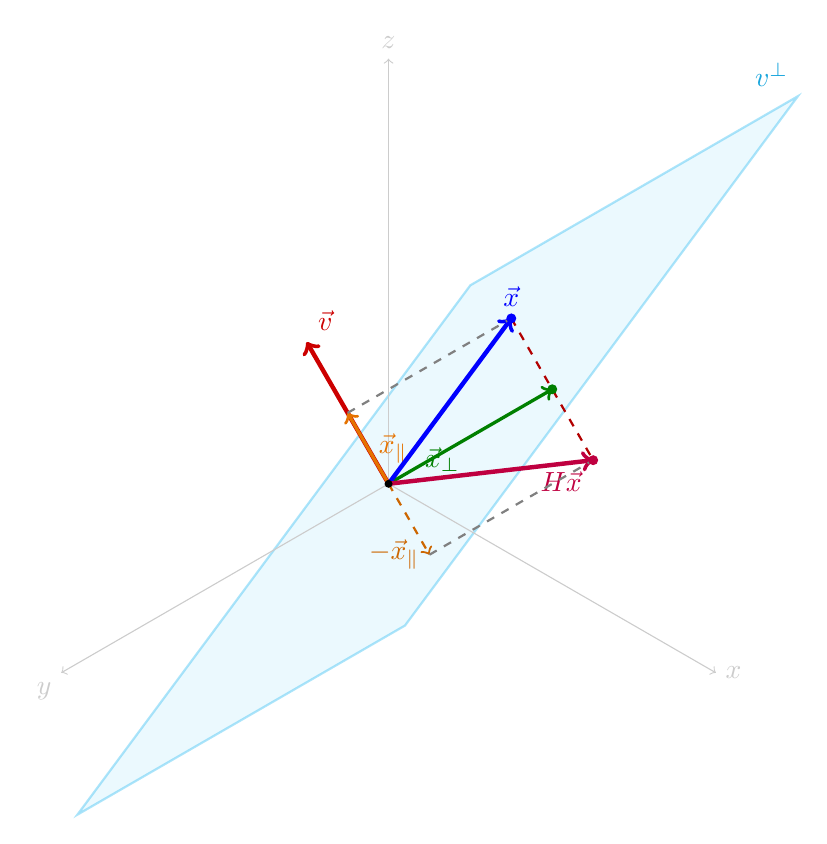
\begin{tikzpicture}[
                x={(0.866cm,-0.5cm)},
                y={(-0.866cm,-0.5cm)},
                z={(0cm,1cm)},
                scale=1.2
            ]
            \coordinate (O) at (0,0,0);
            \coordinate (V) at (1,2,3);
            \coordinate (X) at (2.5,1,3.5);

            % 2. 利用 TikZ 自动计算正交投影 x_parallel = proj_v(x)
            \coordinate (Xpara) at ($ (O)!(X)!(V) $);
            % 3. 计算 x_perp = x - x_parallel
            \coordinate (Xperp) at ($ (X) - (Xpara) $);
            % 4. 计算反射向量 Hx = x_perp - x_parallel = x - 2*x_parallel
            \coordinate (HX) at ($ (X) - 2*(Xpara) $);
            % 计算 -x_parallel 终点 (用于画反向分量)
            \coordinate (NegXpara) at ($ -1*(Xpara) $);
            % 5. 定义超平面内与 V 垂直的第二个方向向量 W = (0, -3, 2)
            \coordinate (W) at (0,-3,2);
            % 6. 构造超平面 v^\perp 的 4 个顶点
            \coordinate (P1) at ($ (O) + 1.3*(Xperp) + 0.8*(W) $);
            \coordinate (P2) at ($ (O) - 0.7*(Xperp) + 0.8*(W) $);
            \coordinate (P3) at ($ (O) - 0.7*(Xperp) - 0.8*(W) $);
            \coordinate (P4) at ($ (O) + 1.3*(Xperp) - 0.8*(W) $);
            % 7. 绘制半透明超平面 v^\perp (镜面)
            \filldraw[fill=cyan!20, draw=cyan!80, opacity=0.4, line width=0.8pt]
            (P1) -- (P2) -- (P3) -- (P4) -- cycle;
            \node[cyan!90!black, above left] at (P1) {\(v^{\perp}\)};
            % 8. 绘制坐标轴 (浅灰色背景)
            \draw[->, gray!40] (O) -- (4,0,0) node[right] {\(x\)};
            \draw[->, gray!40] (O) -- (0,4,0) node[below left] {\(y\)};
            \draw[->, gray!40] (O) -- (0,0,4.5) node[above] {\(z\)};
            % 9. 绘制法向量 v (红色)
            \draw[->, ultra thick, red!80!black] (O) -- (V) node[above right] {\(\vec{v}\)};
            % 10. 绘制正向法向分量 x_parallel 与 反向法向分量 -x_parallel
            \draw[->, very thick, orange!90!black] (O) -- (Xpara) node[midway, right] {\(\vec{x}_{\parallel}\)};
            \draw[->, thick, orange!80!black, dashed] (O) -- (NegXpara) node[left] {\(-\vec{x}_{\parallel}\)};
            % 11. 绘制切向分量 x_perp (绿色，完全平贴在超平面内)
            \draw[->, very thick, green!50!black] (O) -- (Xperp) node[midway, below left] {\(\vec{x}_{\perp}\)};
            % 12. 绘制【原向量 x】 (深蓝色)
            \draw[->, ultra thick, blue] (O) -- (X) node[above] {\(\vec{x}\)};
            % 13. 绘制【反射向量 Hx】 (紫色)
            \draw[->, ultra thick, purple] (O) -- (HX) node[below left] {\(H\vec{x}\)};
            \draw[dashed, thick, gray] (Xpara) -- (X);
            \draw[dashed, thick, gray] (NegXpara) -- (HX);
            % 连接 x 和 Hx 的垂直贯穿线 (穿过 Xperp)
            \draw[dashed, thick, red!70!black] (X) -- (HX);

            \fill[black] (O) circle (1.2pt);
            \fill[blue] (X) circle (1.5pt);
            \fill[purple] (HX) circle (1.5pt);
            \fill[green!50!black] (Xperp) circle (1.5pt);

        \end{tikzpicture}
    \end{figure}

    3: 设计 H  \\
    现给定 : \\
    \begin{align}
        x \in \mathbb{R}^{m}
    \end{align}
    我们希望找到一个反射矩阵 H, 使:
    \begin{align}
        Hx = \alpha e_{1}             \\
        e_{1} = [1, 0, 0, ..., 0]^{T} \\
    \end{align}

    这里我们要先捋清楚几个细节: \\
    反射矩阵是基于超平面 $\vec{v}^{\perp}$ 会存在一个 法向量 $\vec{v} (v \in \mathbb{R}^{m})$ \\
    简单的来说我们需要知道也给 $\vec{v}$ 向量 它可以推导反射矩阵 H (基于 $\vec{v}^{\perp}$) \\
    使其构建下列关键代数式: \\
    \begin{align}
        \alpha e_{1} = y \\
        Hx = y           \\
    \end{align}

    我们现在虽然不知道  $\vec{v}^{\perp}$ 超平面的位置关系, 但我们知道反射有几个重要的性质: \\
    \begin{align}
        ||x|| = ||y|| \;  \text{长度不变性} \\
    \end{align}
    这里我们可以构建一个等腰三角形 $\Delta X0Y$

    \begin{figure}[htbp]
        \centering
        \begin{tikzpicture}[
                x={(0.866cm,-0.5cm)},
                y={(-0.866cm,-0.5cm)},
                z={(0cm,1cm)},
                scale=1.2
            ]

            \draw[->] (0,0,0) -- (5,0,0) node[right] {\(x\)};
            \draw[->] (0,0,0) -- (0,5,0) node[below left] {\(y\)};
            \draw[->] (0,0,0) -- (0,0,5) node[above] {\(z\)};

            \coordinate (O) at (0,0,0);
            \coordinate (X) at (1,2,3);
            \coordinate (Y) at ({sqrt(1*1 + 2*2 + 3*3)}, 0, 0);

            \draw[->, thick, blue] (0,0,0) -- (X) node[above right] {\(\vec{x}\)};
            \draw[->, thick, blue] (0,0,0) -- (Y) node[below] {\(\vec{y}=\sqrt{14}\,\vec{e}_1\)};
            \draw[->, thick, red] (Y) -- (X) node[midway, sloped, above] {\(\vec{v} = \vec{x}-\vec{y}\)};
        \end{tikzpicture}
    \end{figure}

    这里我们从图中能明白得到一个向量 $\vec{v} = \vec{x} - \vec{y}$ \\
    那么我们思考一个问题 这个 $\vec{v}$ 和我们希望得到的 H 的关系是什么呢 ? \\
    我们确定这个 $\vec{v}$ 的身份 它是 "法向量" \\
    那么 使用 关于 H 推导 :\\
    设: $x, y \in \mathbb{R}^{n}$, 且满足: \\
    \begin{align}
        ||x|| = ||y||   \Longleftrightarrow  x^{T}x  = y^{T}y \; (||x||^{2} = ||y||^{2})
    \end{align}
    令: \\
    \begin{align}
        v = x - y  \; (v \neq 0, x \neq y)
    \end{align}
    H 矩阵定义: \\
    \begin{align}
        H = I - 2\frac{vv^{T}}{v^{T}v}
    \end{align}
    其中 $v^{T}v$ 是内积标量, $vv^{T}$ 是 $n \times n$ 外积矩阵 \\
    关于 $Hx = y$ \\
    \begin{align}
        Hx = (I - 2\frac{vv^{T}}{v^{T}v})x           \\
        = (I - \frac{2}{v^{T}v}vv^{T})x              \\
        =  x - \frac{2}{v^{T}v}vv^{T}x               \\
        =  x - \frac{2}{v^{T}v}v(v^{T}x)             \\
        =  x - \frac{2}{v^{T}v}(x-y)((x - y)^{T}x)   \\
        = x - \frac{2}{v^{T}v}(x-y)(x^{T}x - y^{T}x) \\
    \end{align}
    化简 $v^{T}v$ \\
    \begin{align}
        v^{T}v = (x - y)^{T}(x - y)                 \\
        = (x^{T} - y^{T})(x - y)                    \\
        = x^{T}x - x^{T}y - y^{T}x + y^{T}y         \\
        \because x^{T}y = y^{T}x , x^{T}x =  y^{T}y \\
        = 2x^{T}x -2x^{T}y                          \\
        = 2x^{T}v                                   \\
    \end{align}
    \begin{align}
        Hx= x - \frac{2}{v^{T}v}(x-y)(x^{T}x - y^{T}x) \\
        =  x - \frac{2}{2x^{T}v}v(x^{T}x - y^{T}x)     \\
        =  x - \frac{1}{x^{T}v}v(x^{T}x - x^{T}y)      \\
        =  x - v\frac{1}{x^{T}v}(x^{T}v)               \\
        =  x - v                                       \\
        =  x - x + y                                   \\
        = y
    \end{align}
    所以这里我们就能得到一个结论 x, y 建立反射关系是通过 v (由 v 导出 H) \\

    4: 关于$\alpha$ 的符号 \\
    已知 $y = ||x||e1$ 或者  $ y = -||x||e1$ \\
    且 $ v = x - y$ \\
    \begin{align}
        v = x - ||x||e1 \\
        = [x_{1}- ||x||, x_{2}, x_{3}, ...., x_{n}]^{T}
    \end{align}
    我们发现 v 真正存在运算(减法) 的位置只有 $v_{1}$, 并且等于 $x_{1} - ||x||$ \\
    现在存在一个情况: $x_{1} \to ||x||$, $x_{1}$ 无限接近 $||x||$ \\
    那么 $x_{1}- ||x||$ 可能存在计算机科学中浮点运算中会丢失精度 \\
    解决方案是 把 - 转换成 + \\
    这里我们必须要获取到 $x_{1}$ 的符号 $sign(x_{1})$ \\
    把运算转换成:  \\
    \begin{align}
        x_{1} - (-sign(x_{1}))||x||e1) \\
    \end{align}

    5: 计算 \\
    设: \\
    \begin{align}
        x = [4, 3, 0]^{T}              \\
        ||x|| = 5                      \\
        \alpha = -sign(4)||x|| = -5    \\
        y = \alpha e1 = [-5, 0, 0]^{T} \\
        v = x - y = [9, 3, 0]^{T}      \\
    \end{align}
    计算 H :\\
    \begin{align}
        H = I -2\frac{vv^{T}}{v^{T}v}               \\
        =\begin{bmatrix}
             1 & 0 & 0 \\
             0 & 1 & 0 \\
             0 & 0 & 1 \\
         \end{bmatrix} - \frac{1}{45}vv^{T}         \\
        =\begin{bmatrix}
             1 & 0 & 0 \\
             0 & 1 & 0 \\
             0 & 0 & 1 \\
         \end{bmatrix} - \frac{1}{45}\begin{bmatrix}
                                         81 & 27 & 0 \\
                                         27 & 9  & 0 \\
                                         0  & 0  & 0
                                     \end{bmatrix} \\
        =\begin{bmatrix}
             -\frac{4}{5} & -\frac{3}{5} & 0 \\
             -\frac{3}{5} & -\frac{4}{5} & 0 \\
             -0           & 0            & 1 \\
         \end{bmatrix}
    \end{align}
    Check: \\
    \begin{align}
        H = \begin{bmatrix}
                -\frac{4}{5} & -\frac{3}{5} & 0 \\
                -\frac{3}{5} & -\frac{4}{5} & 0 \\
                -0           & 0            & 1 \\
            \end{bmatrix}[4, 3, 0]^{T}            \\
        = [-\frac{16}{5} + -\frac{9}{5} + 0, 0, 0]^{T} \\
        = [-5, 0, 0]^{T}                               \\
    \end{align}






\end{flushleft}
\end{document}